% Created by tikzDevice version 0.9 on 2015-11-20 12:10:21
% !TEX encoding = UTF-8 Unicode
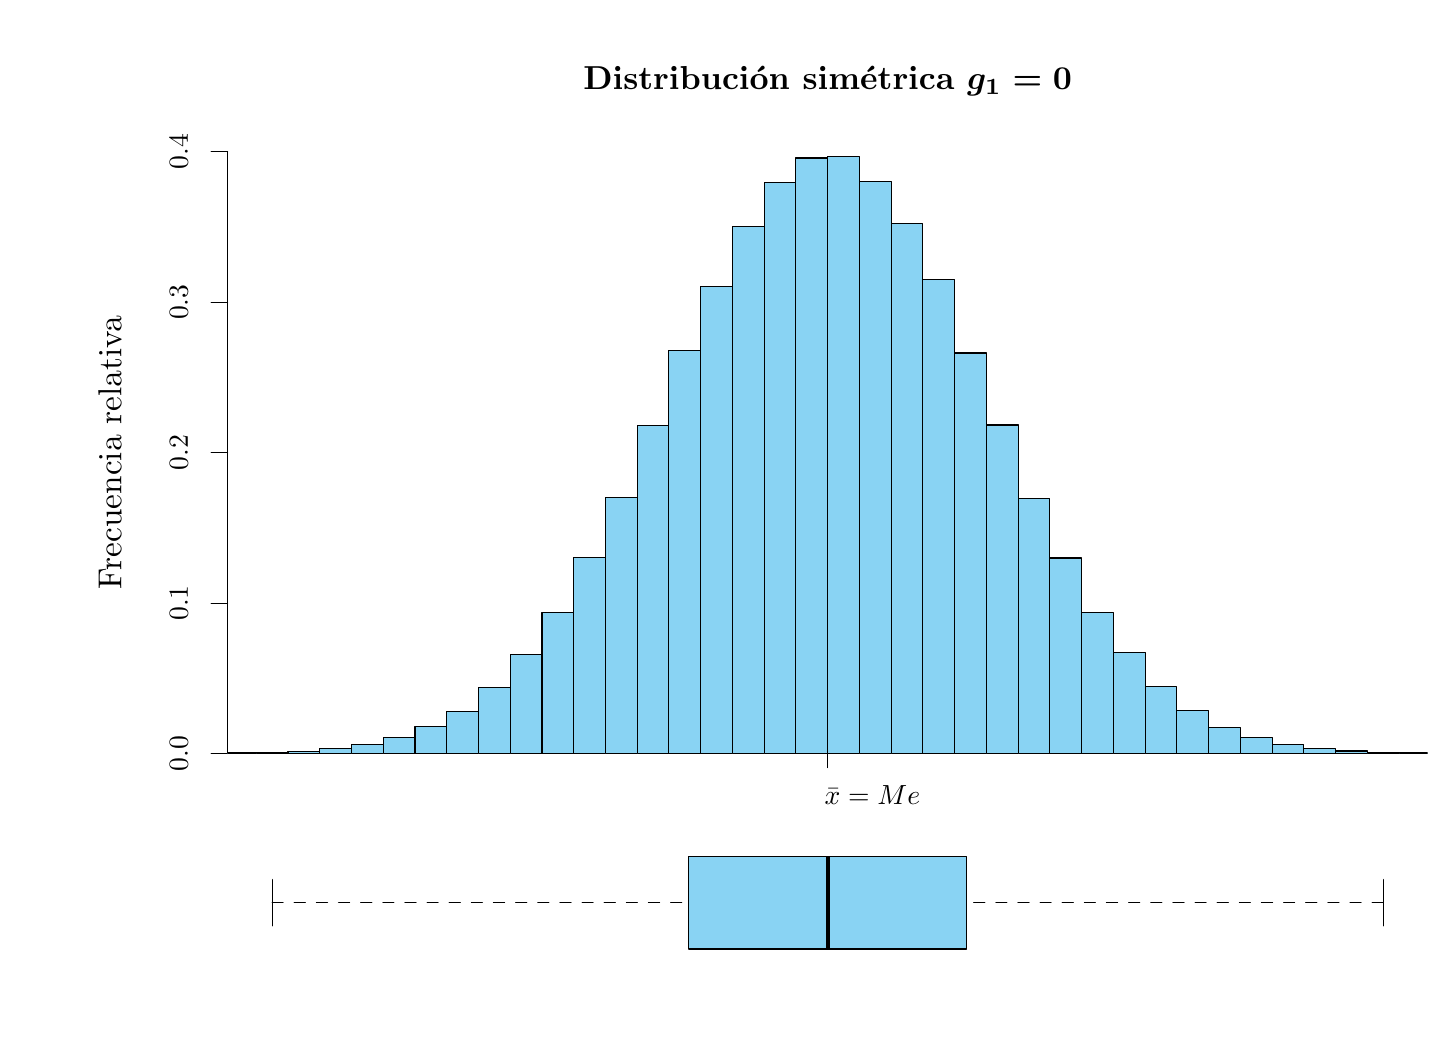
\begin{tikzpicture}[x=1pt,y=1pt]
\definecolor{fillColor}{RGB}{255,255,255}
\path[use as bounding box,fill=fillColor,fill opacity=0.00] (0,0) rectangle (505.89,361.35);
\begin{scope}
\path[clip] (  0.00, 90.34) rectangle (505.89,361.35);
\definecolor{drawColor}{RGB}{0,0,0}

\node[text=drawColor,anchor=base,inner sep=0pt, outer sep=0pt, scale=  1.20, font=\boldmath] at (289.08,339.14)
{\bfseries Distribución simétrica $g_1=0$};
 
\node[text=drawColor,rotate= 90.00,anchor=base,inner sep=0pt, outer sep=0pt, scale=  1.20] at ( 33.87,207.78) {Frecuencia relativa};
\end{scope}
\begin{scope}
\path[clip] (  0.00,  0.00) rectangle (505.89,361.35);
\definecolor{drawColor}{RGB}{0,0,0}

\path[draw=drawColor,line width= 0.4pt,line join=round,line cap=round] ( 72.27, 99.04) -- ( 72.27,316.52);

\path[draw=drawColor,line width= 0.4pt,line join=round,line cap=round] ( 72.27, 99.04) -- ( 66.27, 99.04);

\path[draw=drawColor,line width= 0.4pt,line join=round,line cap=round] ( 72.27,153.41) -- ( 66.27,153.41);

\path[draw=drawColor,line width= 0.4pt,line join=round,line cap=round] ( 72.27,207.78) -- ( 66.27,207.78);

\path[draw=drawColor,line width= 0.4pt,line join=round,line cap=round] ( 72.27,262.15) -- ( 66.27,262.15);

\path[draw=drawColor,line width= 0.4pt,line join=round,line cap=round] ( 72.27,316.52) -- ( 66.27,316.52);

\node[text=drawColor,rotate= 90.00,anchor=base,inner sep=0pt, outer sep=0pt, scale=  1.00] at ( 57.87, 99.04) {0.0};

\node[text=drawColor,rotate= 90.00,anchor=base,inner sep=0pt, outer sep=0pt, scale=  1.00] at ( 57.87,153.41) {0.1};

\node[text=drawColor,rotate= 90.00,anchor=base,inner sep=0pt, outer sep=0pt, scale=  1.00] at ( 57.87,207.78) {0.2};

\node[text=drawColor,rotate= 90.00,anchor=base,inner sep=0pt, outer sep=0pt, scale=  1.00] at ( 57.87,262.15) {0.3};

\node[text=drawColor,rotate= 90.00,anchor=base,inner sep=0pt, outer sep=0pt, scale=  1.00] at ( 57.87,316.52) {0.4};
\end{scope}
\begin{scope}
\path[clip] ( 72.27, 90.34) rectangle (505.89,325.21);
\definecolor{drawColor}{RGB}{0,0,0}
\definecolor{fillColor}{RGB}{137,211,243}

\path[draw=drawColor,line width= 0.4pt,line join=round,line cap=round,fill=fillColor] ( 13.77, 99.04) rectangle ( 25.24, 99.04);

\path[draw=drawColor,line width= 0.4pt,line join=round,line cap=round,fill=fillColor] ( 25.24, 99.04) rectangle ( 36.71, 99.05);

\path[draw=drawColor,line width= 0.4pt,line join=round,line cap=round,fill=fillColor] ( 36.71, 99.04) rectangle ( 48.18, 99.06);

\path[draw=drawColor,line width= 0.4pt,line join=round,line cap=round,fill=fillColor] ( 48.18, 99.04) rectangle ( 59.65, 99.09);

\path[draw=drawColor,line width= 0.4pt,line join=round,line cap=round,fill=fillColor] ( 59.65, 99.04) rectangle ( 71.12, 99.16);

\path[draw=drawColor,line width= 0.4pt,line join=round,line cap=round,fill=fillColor] ( 71.12, 99.04) rectangle ( 82.59, 99.30);

\path[draw=drawColor,line width= 0.4pt,line join=round,line cap=round,fill=fillColor] ( 82.59, 99.04) rectangle ( 94.07, 99.52);

\path[draw=drawColor,line width= 0.4pt,line join=round,line cap=round,fill=fillColor] ( 94.07, 99.04) rectangle (105.54, 99.95);

\path[draw=drawColor,line width= 0.4pt,line join=round,line cap=round,fill=fillColor] (105.54, 99.04) rectangle (117.01,100.89);

\path[draw=drawColor,line width= 0.4pt,line join=round,line cap=round,fill=fillColor] (117.01, 99.04) rectangle (128.48,102.31);

\path[draw=drawColor,line width= 0.4pt,line join=round,line cap=round,fill=fillColor] (128.48, 99.04) rectangle (139.95,104.82);

\path[draw=drawColor,line width= 0.4pt,line join=round,line cap=round,fill=fillColor] (139.95, 99.04) rectangle (151.42,108.79);

\path[draw=drawColor,line width= 0.4pt,line join=round,line cap=round,fill=fillColor] (151.42, 99.04) rectangle (162.89,114.39);

\path[draw=drawColor,line width= 0.4pt,line join=round,line cap=round,fill=fillColor] (162.89, 99.04) rectangle (174.37,123.01);

\path[draw=drawColor,line width= 0.4pt,line join=round,line cap=round,fill=fillColor] (174.37, 99.04) rectangle (185.84,134.71);

\path[draw=drawColor,line width= 0.4pt,line join=round,line cap=round,fill=fillColor] (185.84, 99.04) rectangle (197.31,150.13);

\path[draw=drawColor,line width= 0.4pt,line join=round,line cap=round,fill=fillColor] (197.31, 99.04) rectangle (208.78,169.74);

\path[draw=drawColor,line width= 0.4pt,line join=round,line cap=round,fill=fillColor] (208.78, 99.04) rectangle (220.25,191.61);

\path[draw=drawColor,line width= 0.4pt,line join=round,line cap=round,fill=fillColor] (220.25, 99.04) rectangle (231.72,217.53);

\path[draw=drawColor,line width= 0.4pt,line join=round,line cap=round,fill=fillColor] (231.72, 99.04) rectangle (243.19,244.61);

\path[draw=drawColor,line width= 0.4pt,line join=round,line cap=round,fill=fillColor] (243.19, 99.04) rectangle (254.67,267.97);

\path[draw=drawColor,line width= 0.4pt,line join=round,line cap=round,fill=fillColor] (254.67, 99.04) rectangle (266.14,289.65);

\path[draw=drawColor,line width= 0.4pt,line join=round,line cap=round,fill=fillColor] (266.14, 99.04) rectangle (277.61,305.28);

\path[draw=drawColor,line width= 0.4pt,line join=round,line cap=round,fill=fillColor] (277.61, 99.04) rectangle (289.08,314.26);

\path[draw=drawColor,line width= 0.4pt,line join=round,line cap=round,fill=fillColor] (289.08, 99.04) rectangle (300.55,314.91);

\path[draw=drawColor,line width= 0.4pt,line join=round,line cap=round,fill=fillColor] (300.55, 99.04) rectangle (312.02,305.72);

\path[draw=drawColor,line width= 0.4pt,line join=round,line cap=round,fill=fillColor] (312.02, 99.04) rectangle (323.49,290.70);

\path[draw=drawColor,line width= 0.4pt,line join=round,line cap=round,fill=fillColor] (323.49, 99.04) rectangle (334.97,270.37);

\path[draw=drawColor,line width= 0.4pt,line join=round,line cap=round,fill=fillColor] (334.97, 99.04) rectangle (346.44,243.80);

\path[draw=drawColor,line width= 0.4pt,line join=round,line cap=round,fill=fillColor] (346.44, 99.04) rectangle (357.91,217.79);

\path[draw=drawColor,line width= 0.4pt,line join=round,line cap=round,fill=fillColor] (357.91, 99.04) rectangle (369.38,191.33);

\path[draw=drawColor,line width= 0.4pt,line join=round,line cap=round,fill=fillColor] (369.38, 99.04) rectangle (380.85,169.70);

\path[draw=drawColor,line width= 0.4pt,line join=round,line cap=round,fill=fillColor] (380.85, 99.04) rectangle (392.32,150.03);

\path[draw=drawColor,line width= 0.4pt,line join=round,line cap=round,fill=fillColor] (392.32, 99.04) rectangle (403.79,135.51);

\path[draw=drawColor,line width= 0.4pt,line join=round,line cap=round,fill=fillColor] (403.79, 99.04) rectangle (415.27,123.17);

\path[draw=drawColor,line width= 0.4pt,line join=round,line cap=round,fill=fillColor] (415.27, 99.04) rectangle (426.74,114.54);

\path[draw=drawColor,line width= 0.4pt,line join=round,line cap=round,fill=fillColor] (426.74, 99.04) rectangle (438.21,108.56);

\path[draw=drawColor,line width= 0.4pt,line join=round,line cap=round,fill=fillColor] (438.21, 99.04) rectangle (449.68,104.81);

\path[draw=drawColor,line width= 0.4pt,line join=round,line cap=round,fill=fillColor] (449.68, 99.04) rectangle (461.15,102.37);

\path[draw=drawColor,line width= 0.4pt,line join=round,line cap=round,fill=fillColor] (461.15, 99.04) rectangle (472.62,100.87);

\path[draw=drawColor,line width= 0.4pt,line join=round,line cap=round,fill=fillColor] (472.62, 99.04) rectangle (484.09, 99.97);

\path[draw=drawColor,line width= 0.4pt,line join=round,line cap=round,fill=fillColor] (484.09, 99.04) rectangle (495.57, 99.57);

\path[draw=drawColor,line width= 0.4pt,line join=round,line cap=round,fill=fillColor] (495.57, 99.04) rectangle (507.04, 99.27);
\end{scope}
\begin{scope}
\path[clip] (  0.00,  0.00) rectangle (505.89,361.35);
\definecolor{drawColor}{RGB}{0,0,0}

\path[draw=drawColor,line width= 0.4pt,line join=round,line cap=round] (289.15, 99.04) -- (289.15, 94);

\node[text=drawColor,anchor=west,inner sep=0pt, outer sep=0pt, scale=  1.00] at (288, 84) {$\bar x=Me$};
\end{scope}
\begin{scope}
\path[clip] ( 72.27,  0.00) rectangle (505.89, 90.34);
\definecolor{fillColor}{RGB}{137,211,243}

\path[fill=fillColor] (238.87, 28.44) --
	(238.87, 61.90) --
	(339.25, 61.90) --
	(339.25, 28.44) --
	cycle;
\definecolor{drawColor}{RGB}{0,0,0}

\path[draw=drawColor,line width= 1.2pt,line join=round] (289.15, 28.44) -- (289.15, 61.90);

\path[draw=drawColor,line width= 0.4pt,dash pattern=on 4pt off 4pt ,line join=round,line cap=round] ( 88.33, 45.17) -- (238.87, 45.17);

\path[draw=drawColor,line width= 0.4pt,dash pattern=on 4pt off 4pt ,line join=round,line cap=round] (489.83, 45.17) -- (339.25, 45.17);

\path[draw=drawColor,line width= 0.4pt,line join=round,line cap=round] ( 88.33, 36.80) -- ( 88.33, 53.53);

\path[draw=drawColor,line width= 0.4pt,line join=round,line cap=round] (489.83, 36.80) -- (489.83, 53.53);

\path[draw=drawColor,line width= 0.4pt,line join=round,line cap=round] (238.87, 28.44) --
	(238.87, 61.90) --
	(339.25, 61.90) --
	(339.25, 28.44) --
	(238.87, 28.44);
\end{scope}
\end{tikzpicture}
